\chapter{Stand der Technik} \label{ch_StandTechnik}
Das nachfolgende Kapitel zum Stand der Technik soll alle relevanten Grundlagen bezüglich der verwendeten Komponenten am Solarturm schaffen.
Darüber hinaus wird auch ein Einblick in die Theorie der modellprädiktiven Regelung gegeben.
Ebenfalls relevant ist der Vergleich der verwendeten Zielpunktregelung und des Nowcasting-Systems mit Alternativen aus der Literatur.
Zum Abschluss des Kapitels wird die für diese Arbeit genutzte Hard- und Software vorgestellt.

\section{Solartürme} \label{sec_Solartürme}
Am Forschungszentrum in Jülich ist der Solarturm beheimatet, für den im Rahmen dieser Arbeit eine Regelung entwickelt wird.
Die nachfolgende Abbildung \ref{fig_Solarturm} zeigt diesen 60 Meter hohen Turm \cite{DLRSolartürmeBild}, inklusive der Spiegel, sog. \textit{Heliostaten}, die das Sonnenlicht in Richtung des Receivers fokussieren.

\begin{figure}[h!]
    \centering
    \setlength{\fboxsep}{1pt}
    \setlength{\fboxrule}{1pt}
    \fbox{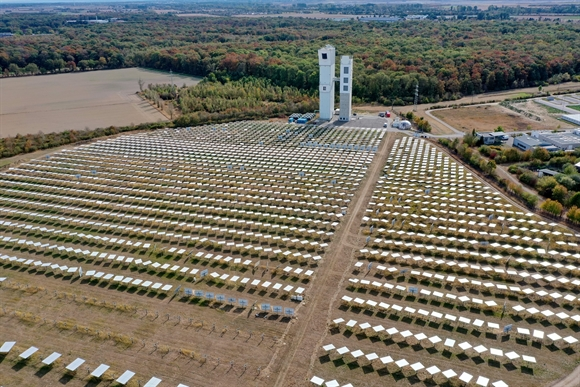
\includegraphics[width=0.7\textwidth]{fig/SolarkraftwerkJuelich.jpg}}
\caption[Solarthermisches Demonstrations- und Versuchskraftwerk Jülich]{Solarthermisches Demonstrations- und Versuchskraftwerk Jülich \cite{DLRSolartürmeBild}}
    \label{fig_Solarturm}
\end{figure}

Ein Solarturmkraftwerk nutzt konzentrierte Sonnenstrahlung für verschiedene Hochtemperaturanwendungen.
Diese konzentrierte Strahlung entsteht durch gezielte Ausrichtung einer großen Anzahl an Heliostaten auf die Spitze des Solarturms, an der sich der \textit{Receiver} befindet.
Dort wird sie von einem Wärmeträgermedium absorbiert, welches anschließend klassischerweise zum Betrieb eines Energieumwandlungsprozesses zur Stromerzeugung verwendet wird.
Alternativ kann das erhitzte Medium auch zur Unterstützung thermochemischer Prozesse genutzt oder in einem Energiespeicher zur späteren Verwendung zwischengespeichert werden. \cite[S.11]{DissBelhomme}\\
Die schematische Darstellung eines Solarturmkraftwerkes zeigt Abbildung \ref{fig_SchemaSolarturmkraftwerk}.

\begin{figure}[h!]
    \centering
    \setlength{\fboxsep}{1pt}
    \setlength{\fboxrule}{1pt}
    \fbox{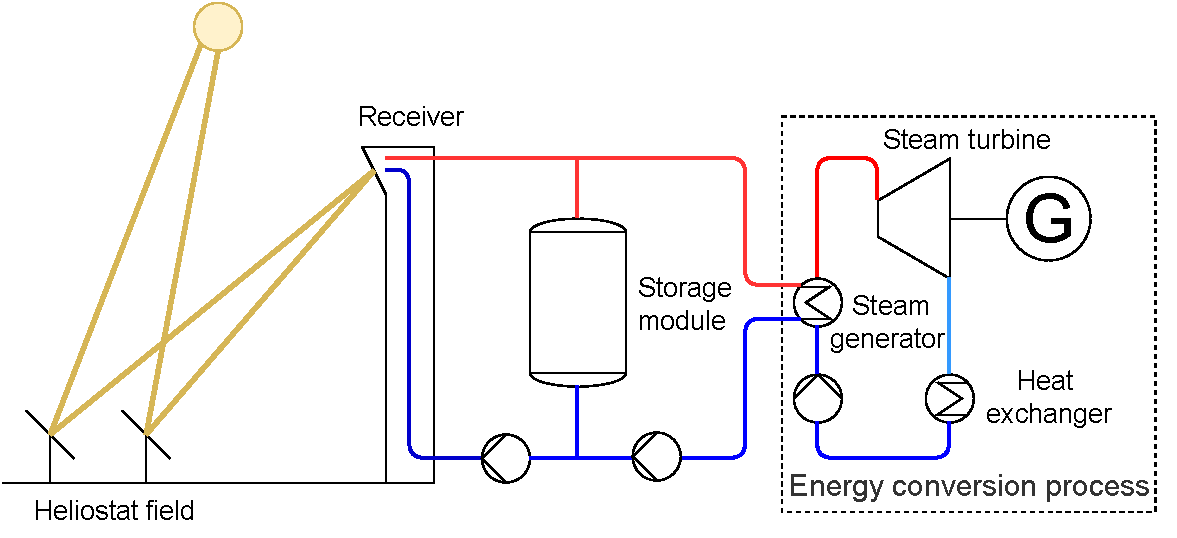
\includegraphics[width=0.9\textwidth]{fig/solar_tower_plant_1.pdf}}
\caption[Vereinfachte schematische Darstellung eines Solarturmkraftwerkes]{Vereinfachte schematische Darstellung eines Solarturmkraftwerkes \cite[S.5]{DissZanger}}
    \label{fig_SchemaSolarturmkraftwerk}
\end{figure}


Da der Fokus dieser Arbeit auf der Front-Temperatur des Receivers sowie der Austrittstemperatur des Mediums auf der Receiver-Innenseite liegt, werden die Komponenten zur Verwertung des Mediums nicht gesondert betrachtet.
Im Gegensatz dazu sind das Heliostatenfeld sowie der Receiver und der Einfluss der Sonneneinstrahlung auf diese Komponenten für das weitere Verständnis der Arbeit durchaus relevant und werden daher nachfolgend in Unterkapiteln näher erläutert.


\subsection{Heliostaten} \label{subsec_Heliostaten}
Die Heliostaten bündeln die Sonneneinstrahlung auf den Receiver.
Dabei bestimmt ihr jeweiliger Zielpunkt, an welcher Stelle der Receiver getroffen wird, sodass sich die Konzentration des Lichtes durch die Nähe der einzelnen Zielpunkte ergibt.

Um seiner Funktion der Sonnenreflexion nachzukommen, besteht jeder Heliostat aus einer reflektierenden Fläche, einer tragenden Struktur und einem Nachführmechanismus.
Letzterer ist erforderlich, um den Receiver auch bei wechselnden Sonnenständen an der jeweils identischen Stelle treffen zu können.
Dafür verfolgt eine integrierte Steuereinheit den Sonnenstand und verstellt die in der Regel bidirektional bewegliche, reflektierende Fläche entsprechend.
Dabei sind die beiden Freiheitsgrade der Heliostaten die Elevations- und die Azimut-Ebene, wie sie in Abbildung \ref{fig_FreiheitsgradeHeliostat} dargestellt sind. \cite[S.13]{DissBelhomme}

\begin{figure}[h!]
    \centering
    \setlength{\fboxsep}{1pt}
    \setlength{\fboxrule}{1pt}
    \fbox{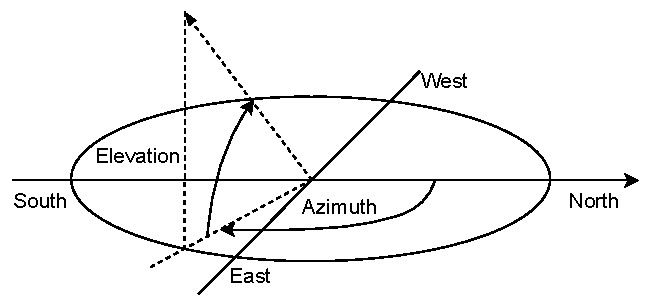
\includegraphics[width=0.7\textwidth]{fig/FreiheitsgradeHeliostat.pdf}}
\caption[Darstellung der Elevations- und Azimut-Ebene]{Darstellung der Elevations- und Azimut-Ebene \cite[S.6]{DissZanger}}
    \label{fig_FreiheitsgradeHeliostat}
\end{figure}

Größe, Form und Art der spiegelnden Fläche unterscheiden sich bei verschiedenen Heliostaten-Typen sehr stark.
Um eine bestimmte Brennweite zu erreichen ist es beispielsweise denkbar die Oberfläche auf kleinere einzelne Flächen, sog. \textit{Facetten}, aufzuteilen, welche sich in einer Ebene oder zueinander gekippt befinden.
Weiterhin sind die Spiegel zumeist rechteckig angeordnet, eine Krümmung der Fläche nach innen, erzielt eine höhere Konzentration der Strahlung. \cite[S.5]{DissZanger}

Der tragende Körper der Heliostaten ist in der Regel aus wirtschaftlichen Gründen als T-Struktur vorgesehen \cite[S.97]{ScottAJones}.
Die Heliostaten am Betrachtungsstandort Jülich bestehen aus lediglich einer ebenen, rechteckigen Facette auf einem T-Träger und sind mit einer Reflexionsfläche von $8.3m^2$ vergleichsweise klein \cite[S.4]{DissGall}\cite[S.13]{DissBelhomme}.
Auf der \textit{PS10} (Planta Solar 10) bei Sevilla befinden sich beispielsweise Heliostaten mit $120m^2$ Reflexionsfläche in 28 Facetten \cite[S.5]{ManuelSilva}.
Die nachfolgende Abbildung \ref{fig_DarstellungHeliostat} soll die grundsätzliche Ähnlichkeit im Aufbau der Heliostaten auch bei unterschiedlicher Größe zeigen.

\begin{figure}[h!]
    \centering
    \setlength{\fboxsep}{1pt}
    \setlength{\fboxrule}{1pt}
    \fbox{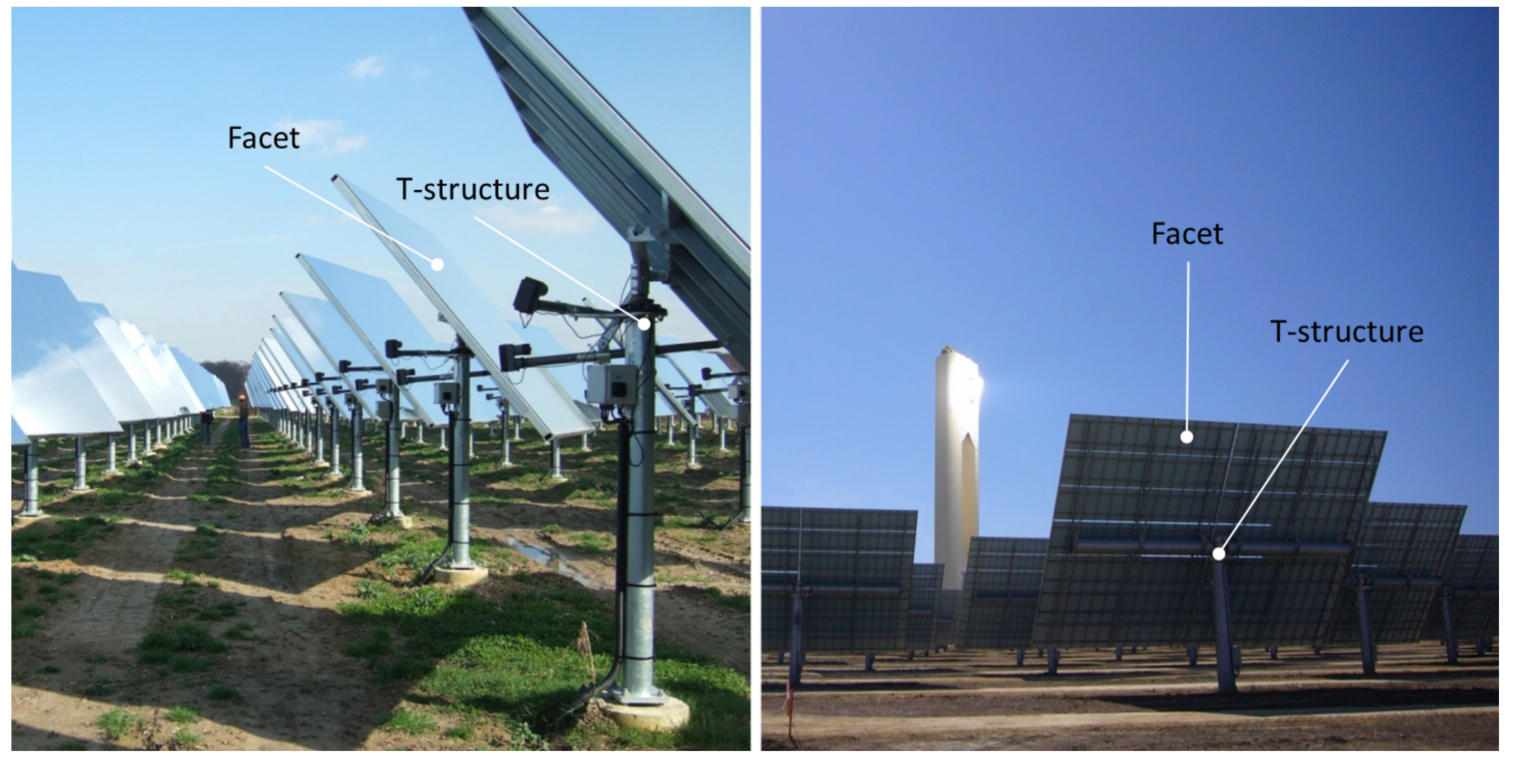
\includegraphics[width=1\textwidth]{fig/Heliostat.png}}
\caption[Ausra Heliostat am Forschungsstandort Jülich mit $8.3m^2$  und Sanlúcar-120-Heliostat auf der PS10 bei Sevilla mit $120m^2$ Reflexionsfläche]{Ausra Heliostat am Forschungsstandort Jülich mit $8.3m^2$  (links) und Sanlúcar-120-Heliostat auf der PS10 bei Sevilla mit $120m^2$ Reflexionsfläche (rechts) \cite[S.13]{DissBelhomme}}
    \label{fig_DarstellungHeliostat}
\end{figure}

Die Gesamtheit der Heliostaten, die um den Receiver eines Solarstromturms angeordnet sind, wird Heliostatenfeld bezeichnet.
Diese bestehen normalerweise aus identischen Heliostaten, welche in Reihen oder konzentrischen Kreisen angeordnet sind.
Denkbare Anordnungen sind Rundum-, Nord- und Südfelder (siehe Abbildung \ref{fig_AnordnungHeliostatfeld}); die effizienteste Anordnung ist jeweils besonders von der geografischen Lage abhängig.
Effektiv sind Solarturmkraftwerke vor allem bei steilen Einfallswinkeln der Sonne auf die Spiegel (vgl. Kapitel \ref{subsubsec_KosinusVerluste}), sodass sich zwangsläufig in Polnähe bei Rundum-Feldern eine geringe Feldausbeute auf einer Seite ergibt.
Wie in Abbildung \ref{fig_Solarturm} zu sehen ist, handelt es sich in Jülich um ein einseitiges, nach Norden ausgerichtetes Feld, bestehend aus 2153 Heliostaten.

\begin{figure}[h!]
    \centering
    \setlength{\fboxsep}{1pt}
    \setlength{\fboxrule}{1pt}
    \fbox{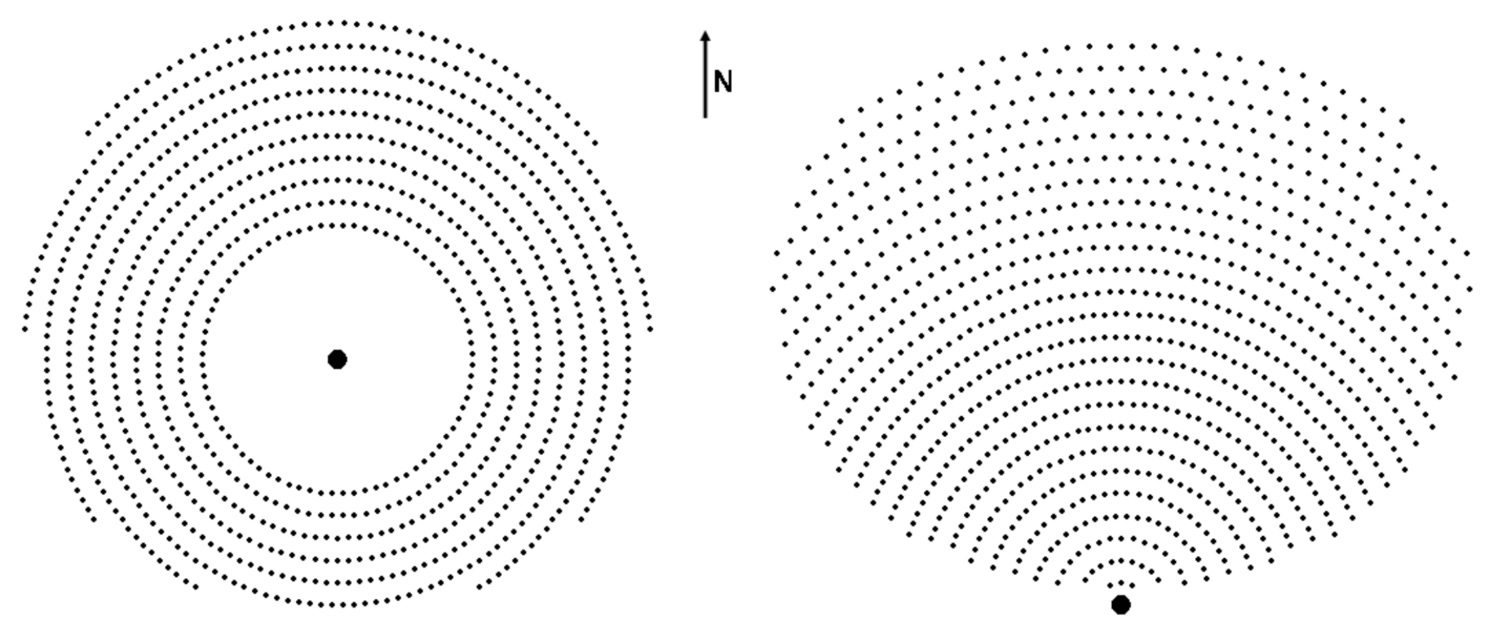
\includegraphics[width=1\textwidth]{fig/Vergleich_Heliostatenfelder.png}}
\caption[Verschiedene Heliostatfeld-Layouts auf der Nordhalbkugel: Rundum-Feld und Nordfeld]{Verschiedene Heliostatfeld-Layouts auf der Nordhalbkugel: Rundum-Feld (links) und Nordfeld (rechts) \cite[S.14]{DissBelhomme}}
    \label{fig_AnordnungHeliostatfeld}
\end{figure}

\subsection{Receiver} \label{subsec_Receiver}

Wie erwähnt ist die Aufgabe des Receivers die Absorption der reflektierten Sonneneinstrahlung oben am Turm.
Durch Konvektion wird die gespeicherte Energie dann an ein Wärmeträgermedium weitergegeben, das dann zur weiteren Verwertung oder Speicherung zur Verfügung steht.
Receiver, die in Solarturmkraftwerken genutzt werden, unterscheiden sich in ihrem Aufbau und ihren physikalischen Grenzen. Diese Eigenschaften werden im Folgenden kurz untersucht.

Grundsätzlich muss zwischen zylindrischen und rechteckigen Receivern unterscheiden werden.
Erstere sind dann notwendig, wenn die Spiegel rund um den Solarturm angeordnet sind. Bei Nord- oder Südfeldern kommen rechteckige Receiver zum Einsatz, welche je nach Standort und Anwendungsfall auch nach innen gebogen sind, um vor Wärmeverlust durch zu schnelle Windgeschwindigkeiten an der Receiver Vorderseite zu schützen. \cite{Flesch}

Das Material des Receivers ist abhängig vom genutzten Wärmeträgermedium.
Typische Medien sind Luft, geschmolzene Salze, Wasser oder flüssige Metalle; die Receiver bestehen in der Regel aus Metallröhren unterschiedlicher Legierungen für den Durchfluss von z.B. Salzschmelzen und Wasser oder aber aus poröser Keramik \cite{Barlev}\cite{Ho2017}.

Wenn Eigenschaften wie die maximal zulässigen thermischen Spannungen des Receivers überschritten werden, kann dieser beschädigt werden \cite{AlbertoSanchez}.
Bei einem Empfänger, der von Salzschmelze durchströmt wird, hängt diese beispielsweise mit der lokalen Salztemperatur und -geschwindigkeit
sowie der Windgeschwindigkeit zusammen \cite{VantHull}.
Dabei wird die lokale Salztemperatur direkt durch die Einstrahlung (Flussdichte) auf dem Receiver beeinflusst.

Eine Möglichkeit die Einhaltung der maximalen thermischen Spannungen zu gewährleisten ist also unter anderem die Einführung einer maximalen Flussdichte am Receiver, die auf der Grundlage seiner spezifischen Eigenschaften berechnet werden kann.
Dabei ist der zulässige Wert auch stark vom verwendeten Kühlmedium abhängig.
Für Röhrenreceiver, die mit flüssigem Natrium gekühlt werden, sind beispielsweise maximale Strahlungsflussdichten von $2,5MW/m^2$ erlaubt, während bei luftgekühlten Röhrenreceivern nur $200kW/m^2$ \cite[S.17]{DissBelhomme} erreicht werden dürfen.

Die Flussdichte $\phi$ ist dabei als Strahlungsfluss $F$ pro Fläche $A$ zu verstehen, wobei $F$ das Verhältnis aus absorbierter Strahlungsenergie $Q$ pro Zeiteinheit darstellt (siehe Formel \ref{eq_Strahlungsfluss} und \ref{eq_Flussdichte}).

\begin{equation} \label{eq_Strahlungsfluss}
    F = \frac{\text{d}Q}{\text{d} t}
\end{equation}
\centerline{\small{\textsf{\textbf{Formel \ref{eq_Strahlungsfluss}:}} Berechnung des Strahlungsflusses $F$}}
\myequations{\quad Berechnung des Strahlungsflusses $F$}

\begin{equation} \label{eq_Flussdichte}
    \phi = \frac{\text{d}F}{\text{d} A}
\end{equation}
\centerline{\small{\textsf{\textbf{Formel \ref{eq_Flussdichte}:}} Berechnung der Flussdichte $\phi$}}
\myequations{\quad Berechnung der Flussdichte $\phi$}

Zur Bestimmung der Brutto-Leistung, die dem System auf diese Weise zugeführt wird, kann die Flussdichte an jeder Receiveröffnung zur Hilfe genommen werden.
Sie ergibt sich aus der Integration der Flussdichte $\phi$ über der Fläche des Receivers (siehe Formel \ref{eq_LeistungReceiver})

\begin{equation} \label{eq_LeistungReceiver}
    P = \int_{A}\phi~\text{d} A
\end{equation}
\centerline{\small{\textsf{\textbf{Formel \ref{eq_LeistungReceiver}:}} Berechnung Bruttoleistung $P$ auf dem Receiver}}
\myequations{\quad Berechnung Bruttoleistung $P$ auf dem Receiver}

Es ist durchaus vorstellbar, dass je nach Anwendungsfall auch ein Limit für die minimal erlaubte Flussdichte auf dem Receiver existiert, um beispielsweise ein Problem von Verfestigung von Salzschmelzen zu vermeiden.
Da das in dieser Arbeit untersuchte Turmkraftwerk in Jülich jedoch mit einem ebenen, rechteckigen Receiver aus Keramik und mit Luftkühlung ausgestattet ist, wird dies an hier nicht weiter betrachtet.
Die vorliegenden Einschränkungen bezüglich thermischen Maximalbelastungen des Receivers werden dem Betriebshandbuch entnommen.
Dort wird die maximale lokale Temperatur der Absorberfläche, welche offensichtlich direkt von der Flussdichte $\phi$ abhängig ist, mit $1273.15K$ angegeben \cite{HandbuchJülich}. Dieser Wert dient in den nachfolgenden Simulationen in Kapitel \ref{ch_AnalyseRegelung} als Indikator für eine erfolgreiche Regelung, welche die Einhaltung dieses Limits als Grundvoraussetzung beinhaltet.

\subsection{Optische Verluste} \label{subsec_OptischeVerluste}
Um den effizientesten Betrieb solarer Turmkraftwerke zu erreichen, ist die Minimierung optischer Verluste wesentlich.
Diese optischen Verluste sind einerseits geografischer Natur, aber auch durch die Wirkweise der Heliostaten bedingt und werden nachfolgend kurz erläutert.
Auf meteorologische Einflüsse wird in Kapitel \ref{sec_Nowcasting} näher eingegangen.

\subsubsection*{Kosinus-Verluste} \label{subsubsec_KosinusVerluste}
Die \textit{Kosinus-Verluste} sind ein besonders schwerwiegender Einflussfaktor geografischer Natur.
Die Sonnenstrahlen treffen auf die Spiegeloberfläche unter einem bestimmten Winkel, der davon abhängt, wo die Sonne steht und wie der Spiegel ausgerichtet ist.
Dieser Winkel bestimmt die effektive Reflexionsfläche, welche senkrecht zur Einfallsrichtung der Strahlung projiziert wird.
Wie in Abbildung \ref{fig_KosinusVerlust} dargestellt ist, entspricht das Verhältnis zwischen der effektiven Fläche und der Gesamtfläche jedes Heliostaten dem Kosinus des Winkels zwischen der Einfallsrichtung und der Hauptnormalen der Spiegelfläche.
Bei zunehmendem Winkel $\beta$ größer wird, also ungünstigeren Lichteinfallswinkeln, nimmt die effektive Fläche ab und die Effizienz der Heliostaten wird geringer.
Diese wird mit dem Kosinus-Wirkungsgrad $\cos\beta$ ausgedrückt, der also in direktem Zusammenhang mit der reflektierten Sonnenleistung steht.
Der immense Einfluss der Kosinus-Verluste zeigt sich beispielsweise an Untersuchungen am Solar One Tower in Süd-Kalifornien, wo auch das Solarturmkraftwerk mit der höchsten Nennleistung beheimatet ist \cite{Ivanpah}.
Zwischen $0,65$ und $0,9$ schwankt der Kosinus-Wirkungsgrad jährlich in dieser Gegend, je nach Sonnenstand und damit verbundener Heliostaten Position. \cite{Holl}

\begin{figure}[h!]
    \centering
    \setlength{\fboxsep}{1pt}
    \setlength{\fboxrule}{1pt}
    \fbox{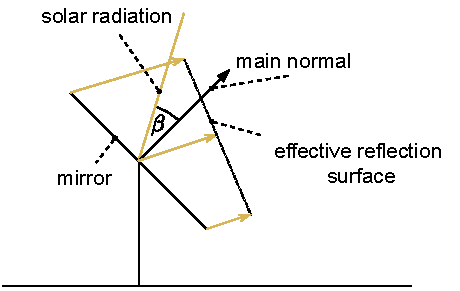
\includegraphics[width=0.6\textwidth]{fig/KosinusVerluste}}
\caption[Seitenansicht eines Heliostaten zur Verdeutlichung des Winkels $\beta$ im Kontext der Kosinus-Verluste]{Seitenansicht eines Heliostaten zur Verdeutlichung des Winkels $\beta$ im Kontext der Kosinus-Verluste \cite[S.7]{DissZanger}}
    \label{fig_KosinusVerlust}
\end{figure}

\subsubsection*{Reflexionsverluste} \label{subsubsec_Reflexionsverluste}
Als schwerwiegender optischer Verlust durch die Heliostaten an sich ist der \textit{Reflexionsverlust} zu nennen.
Wenn das Sonnenlicht auf die Spiegel trifft, wird ein Teil davon absorbiert, was die Menge des reflektierten Lichts verringert.
Diese Verringerung des Reflexionsvermögens kann zusätzlich durch Umweltfaktoren wie Regen und Staub noch verstärkt werden.
Reflektieren saubere Spiegeloberflächen normalerweise zwischen $87 \%$ und $94 \%$ des auf sie treffenden Sonnenlichts, sinkt dieser Wert durch umweltbedingte Verschmutzung womöglich bis auf $80 \%$. \cite[S.14]{DissBelhomme}

\subsubsection*{Blockierung und Abschattung} \label{subsubsec_blockingshading}
Je nach Sonnenstand, Feldanordnung und Objekten mit signifikantem Schattenwurf, wie dem Turm, können Heliostaten verschattet werden oder andere Heliostaten \gans{blockieren}.
Im Falle einer \textit{Abschattung} ist der direkte Weg zwischen Sonne und Heliostat (teilweise) versperrt, sodass die Sonnenstrahlung nicht ungehindert auf die Spiegelfläche treffen kann.
Bei der \textit{Blockierung} ist der Weg zwischen Heliostat und Receiver betroffen; die reflektierte Strahlung eines Heliostaten wird durch einen anderen Heliostaten (teilweise) blockiert.
Abbildung \ref{fig_AbschattungBlockieren} stellt die beiden Problematiken visuell dar.
Das Problem der Abschattung tritt besonders bei niedrigen Sonnenständen auf, während von der Blockierung zumeist die hinteren Heliostatenreihen betroffen sind.
Durch ein geeignetes Felddesign kann diesen Verlusten entgegengewirkt werden. \cite[S.686]{Wei2010}

\begin{figure}[h!]
    \centering
    \setlength{\fboxsep}{1pt}
    \setlength{\fboxrule}{1pt}
    \fbox{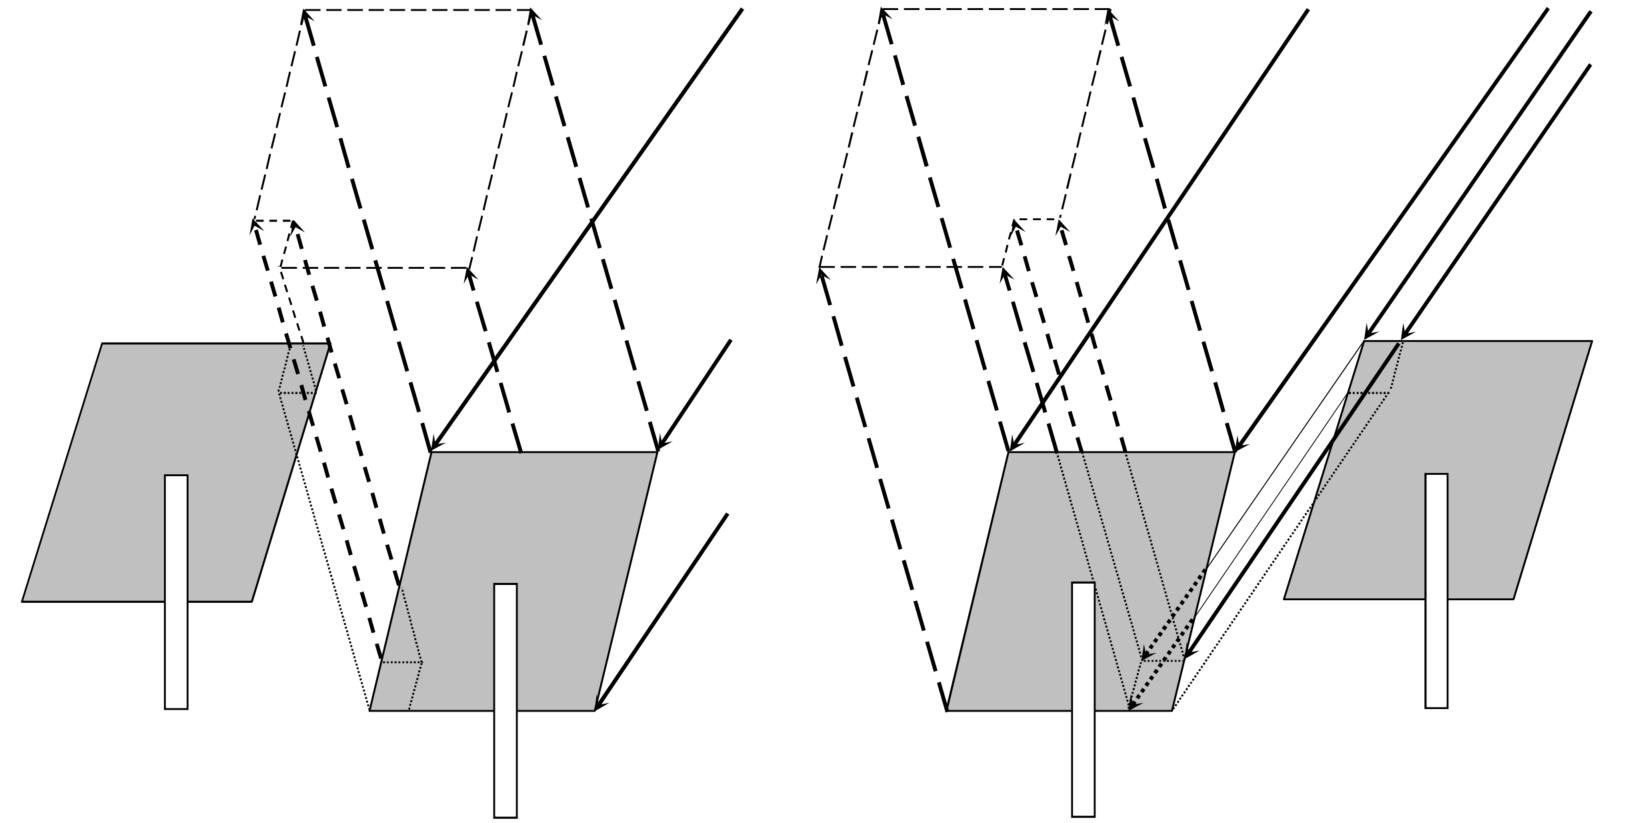
\includegraphics[width=1\textwidth]{fig/BlockingShading.png}}
\caption[Blockierung und Abschattung von Heliostaten]{Blockierung (links) und Abschattung (rechts) von Heliostaten \cite[S.15]{DissBelhomme}}
    \label{fig_AbschattungBlockieren}
\end{figure}

\subsubsection*{Spiegelfehler} \label{subsubsec_Spiegelfehler}
Ein weiterer optischer Verlustfaktor sind die \textit{Spiegelfehler}.
Als solche werden Abweichungen eines Spiegels von seiner idealen Form genannt, welche den Spiegel wellig erscheinen lassen.
Hervorgerufen wird dieser Fehler beispielsweise durch innere Spannungen in der Heliostatenstruktur als Folge von Wind oder Temperaturschwankungen oder aber durch normale Ungenauigkeiten in der Herstellung.
Die Größe des Fehlers wird als Winkel zwischen dem tatsächlichen Normalvektor des Spiegels und dem idealen Normalvektor gemessen und liegt in der Regel zwischen $0,08^\circ$ und $0,14^\circ$. \cite[S.16]{DissBelhomme}

\subsubsection*{Streuung} \label{subsubsec_Streuung}
Als \textit{Streuung} bezeichnet man den Teil der reflektierten Sonnenstrahlung, der den Receiver ungewollt verfehlt und nicht in nutzbare Energie umgewandelt werden kann.
Dies geschieht beispielsweise auch durch die oben genannten Spiegelfehler oder wenn der Abstand zwischen Heliostat und Receiver so groß ist, dass das Abbild der Reflexion auf dem Receiver größer ist als der Receiver selbst. \cite[S.15-16]{DissBelhomme}

\subsubsection*{Nachführfehler} \label{subsubsec_Nachführfehler}
Der letzte nennenswerte optische Fehler, welcher durch die Heliostaten selbst ausgelöst wird, ist der sogenannte \textit{Nachführfehler}.
Dieser beschreibt einen Fehler bei der Ausrichtung der Heliostaten.
Er kann Ursachen wie Schmutz oder Verschleiß an den Nachführachsen, oder Ungenauigkeiten bei der Motorausrichtung und Sonnenstandsmessung als Ursache haben \cite[S.7]{Richter}. Auch dieser Fehler wird als Winkel gemessen und liegt normalerweise bei $0,03^\circ$ bis $0,1^\circ$ \cite[S.17]{DissBelhomme}.

Für die Analyse des Systems wird nachfolgend mit vorberechneten Strahlungskarten aus dem in \cite[S.53ff]{DissBelhomme} vorgestellten Programm \textit{STRAL} verwendet.
Die Software berücksichtigt das reale Heliostatenfeld am Standort Jülich und bietet auch die Möglichkeit optische Verluste zu einem gewissen Grad mit einzubeziehen.


\section{Nowcasting-Systeme zur Wettervorhersage} \label{sec_Nowcasting}
Wie eingangs beschrieben, liegt ein wesentlicher Schwerpunkt dieser Arbeit in der Analyse des Wolkeneinflusses, welcher den besagten meteorologischen optischen Verlust darstellt, auf das Gesamtsystem des Solarturms.
Um eine zuverlässige Regelung hinsichtlich der im Kapitel \ref{subsec_Receiver} beschriebenen Receivertemperaturbegrenzung zu gewährleisten, ist eine möglichst genaue Wolkenvorhersage unerlässlich.
In der Praxis wird dies durch die sogenannten \textit{Nowcasting Systeme} erreicht, die in Ergänzung zu den klassischen Modellen der Wettervorhersage durch zeitlich und räumlich hochauflösende Beobachtungen genauere Vorhersagen liefern \cite{DWD1}.

Die sensorischen Möglichkeiten um solch präzise Vorhersagen generieren zu können sind sehr vielfältig.
Für deutschlandweit flächendeckende Vorhersagen nutzt der deutsche Wetterdienst beispielsweise Radarsysteme und Satellitenbilder \cite{DWD1}.
Durch Abruf und Verarbeitung dieser Daten im 5-Minutentakt können regionale Prognosen für die kommenden zwei Stunden generiert werden.
Diese enthalten dann Informationen über Regenfälle und Hagel, sowie Böen, Blitze und Schneefall.

Für den Anwendungsfall des Solarturms ist eine solche Prognose jedoch aus mehreren Gründen nicht optimal.
Je präziser die jeweils lokale Vorhersage für das Heliostatenfeld ist, desto mehr Information steht der Regelung für eine präzise Regelung zur Verfügung.
Da die Auflösung der deutschlandweiten Vorhersage lediglich rund $1km$ x $1km$ beträgt \cite{DWD1}\cite{DWD2} während sich das Heliostatenfeld auf eine Fläche von rund $330m$ x $310m$ beschränkt, sind lediglich sehr grobe Vorhersagen zu erwarten.
Darüber hinaus ist auch die zeitliche Auflösung von 5 Minuten \cite{DWD2} unterhalb der Möglichkeiten anderer Nowcasting Systeme \cite{DLRNowcasting}\cite[S.272]{QuesadaRuiz}.

Ein beliebtes Instrument für zeitlich und räumlich hochauflösende Vorhersagen sind die sogenannten \textit{ASIs}, kurz für \gans{All-sky imagers}.
Dabei handelt es sich um nach oben gerichtete Kameras mit dem Zweck der Wolkenüberwachung.
Der Prozess zur Erstellung von Nowcasting Vorhersagen auf Basis dieser Bilder wird beispielsweise von Quesada-Ruiz et al. in \cite{QuesadaRuiz} beschrieben. \cite{Samu}

Das DLR verwendet in Spanien bereits ein Nowcasting System auf Basis der ASIs.
Es erstellt in subminütlicher Auflösung Einstrahlungskarten des betrachteten Solarfeldes.
Räumlich gesehen können auf diese Weise Vorhersagen auf bis zu $20m$ x $20m$ getroffen werden. \cite[S.13]{Samu}\cite{DLRNowcasting}

Die nachfolgende Abbildung \ref{fig_Nowcasting_Kamerabilder} zeigt links exemplarisch Bilder, die von solchen ASIs auf der PSA (Plataforma Solar de Almería) in Spanien, einem weiteren Standort eines Solarturmkraftwerkes, entstanden sind.
Für die Erstellung dieser konkreten Bilder wurden 4 Kameras mit jeweils $500$ bis $1000m$ Entfernung voneinander am Heliostatenfeld aufgestellt.
Aus diesen können anschlißend die in Abbildung \ref{fig_Nowcasting_Kamerabilder} rechts sichtbaren Wolkenmasken erstellt und damit die benötigten hochauflösenden Einstrahlungskarten berechnet werden. \cite{DLRNowcasting}

\begin{figure}[h!]
    \centering
    \setlength{\fboxsep}{1pt}
    \setlength{\fboxrule}{1pt}
    \fbox{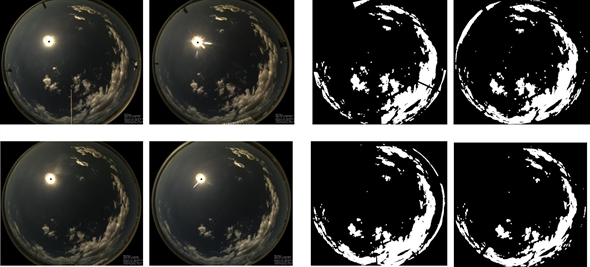
\includegraphics[width=1\textwidth]{fig/Nowcasting}}
\caption[Aufnahmen der ASIs auf der PSA  und die daraus extrahierten Wolknemaske]{Aufnahmen der ASIs auf der PSA (links) und die daraus extrahierten Wolknemasken (rechts) \cite{DLRNowcasting}}
    \label{fig_Nowcasting_Kamerabilder}
\end{figure}


\section{Modellprädiktive Regelung} \label{sec_ModellprädiktiveRegelung}
Das Ziel eines Reglers ist im Allgemeinen, bestimmte Modellparameter, meist Ausgangsgrößen technischer Prozesse, so einzustellen, dass sie vorgegebenen Führungsgrößen entsprechen.
Änderungen dieser Führungsgrößen soll möglichst genau gefolgt werden und unvorhersehbare Störungen sollen die Regelstrecke so wenig wie möglich beeinflussen. \cite{Abel} \\
Im Anwendungsfall dieser Arbeit ist dabei von besonderer Bedeutung, dass auch zukünftige Modellzustände in die Regelung prädiktiv einbezogen werden können.
Aus diesem Grund sind klassische Regler wie der PID Regler, die lediglich auf Basis der Abweichung von aktuellen Soll- und Istwerten Stellgrößen für das System vorgeben \cite[S.408]{Lunze}, nicht ausreichend und es wird ein modellprädiktiver Regler (kurz \textit{MPC}) gewählt.

\subsection{Grundlagen} \label{subsec_GrundlagenMPC}
Neben der Möglichkeit zur Inbezugnahme von Vorhersagen ist ein großer Vorteil der MPC die Fähigkeit komplexe nicht-lineare \textit{MIMO}-Systeme (\textbf{M}ulti \textbf{I}nput \textbf{M}ulti \textbf{O}utput) ohne besonders hohen Aufwand zu regeln.
Der wohl bedeutendste Grund dafür, dass MPC in der Praxis mit dem PID-Regler den Stand der Technik ausmacht \cite[S.viii]{Kouvaritakis}, ist jedoch die zusätzliche Möglichkeit Limitierungen auf Inputs und Outputs des Systems, sogenannte \textit{Constraints}, festlegen zu können; nachteilig ist jedoch der damit direkt verbundene, hohe Rechenaufwand. \cite[S.1-2]{Kouvaritakis}

Der Grund für diese besonderen Features des MPC sind in seinem Aufbau zu finden.
Der Controller an sich besteht aus einer Komposition einer Optimierungseinheit und einem Modell des zu regelnden Systems.
Je präziser das zu regelnde Realmodell in der Modellbildung (vgl. Kapitel \ref{subsec_Modellbildung}) mathematisch beschrieben wird, desto genauer werden logischerweise auch die Ergebnisse der Regelung.
Abbildung \ref{fig_RegelkreisMPC} zeigt den Aufbau eines Regelkreises mit dem MPC.
Für die konkrete Anwendung würde der Solarturm die Anlage (\gans{Plant}) darstellen, in dieser Arbeit wird jedoch nur ein Modell dessen simuliert.

\begin{figure}[h!]
    \centering
    \setlength{\fboxsep}{1pt}
    \setlength{\fboxrule}{1pt}
    \fbox{\includegraphics[width=1\textwidth]{fig/Regelkreis.drawio.pdf}}
\caption[Geschlossener Regelkreis mit einem MPC]{Geschlossener Regelkreis mit einem MPC gemäß\cite[S.2]{Schwenzer}}
    \label{fig_RegelkreisMPC}
\end{figure}

Zum besseren Verständnis des Funktionsprinzips eines modellprädiktiven Reglers dient die nachfolgende Abbildung \ref{fig_MPCVerhalten}.
Es ist erkennbar, dass der Regler zum Zeitpunkt $k$ über die Dauer des gesamten \textit{Prädiktionshorizontes} $N_2$ mittels des hinterlegten Modells die Ausgangsgröße $y$ simuliert.
Die Berechnung geschieht dabei in der durch die \textit{Sample Time} $T_s$ vorgegebenen Frequenz.
Dafür kalkuliert er für den \textit{Regelungshorizont} von Zeitpunkt $k+N_1$ bis $k+N_u$ die optimalen Stellgrößen $u$, sodass sich $y$ der Referenztrajektorie $r$ so gut wie möglich annähert.
Der Abstand zwischen der Referenztrajektorie und der Ausgangsgröße wird mit dem Fehler $e$ bezeichnet, den es zu minimieren gilt.
Nach jedem Zeitschritt $T_s$ verschieben sich die Horizonte entsprechend, es wird eine neue Stellgröße an das System weitergegeben und die Optimierung wird erneut durchgeführt. \cite[S.3]{Schwenzer}

\begin{figure}[h!]
    \centering
    \setlength{\fboxsep}{1pt}
    \setlength{\fboxrule}{1pt}
    \fbox{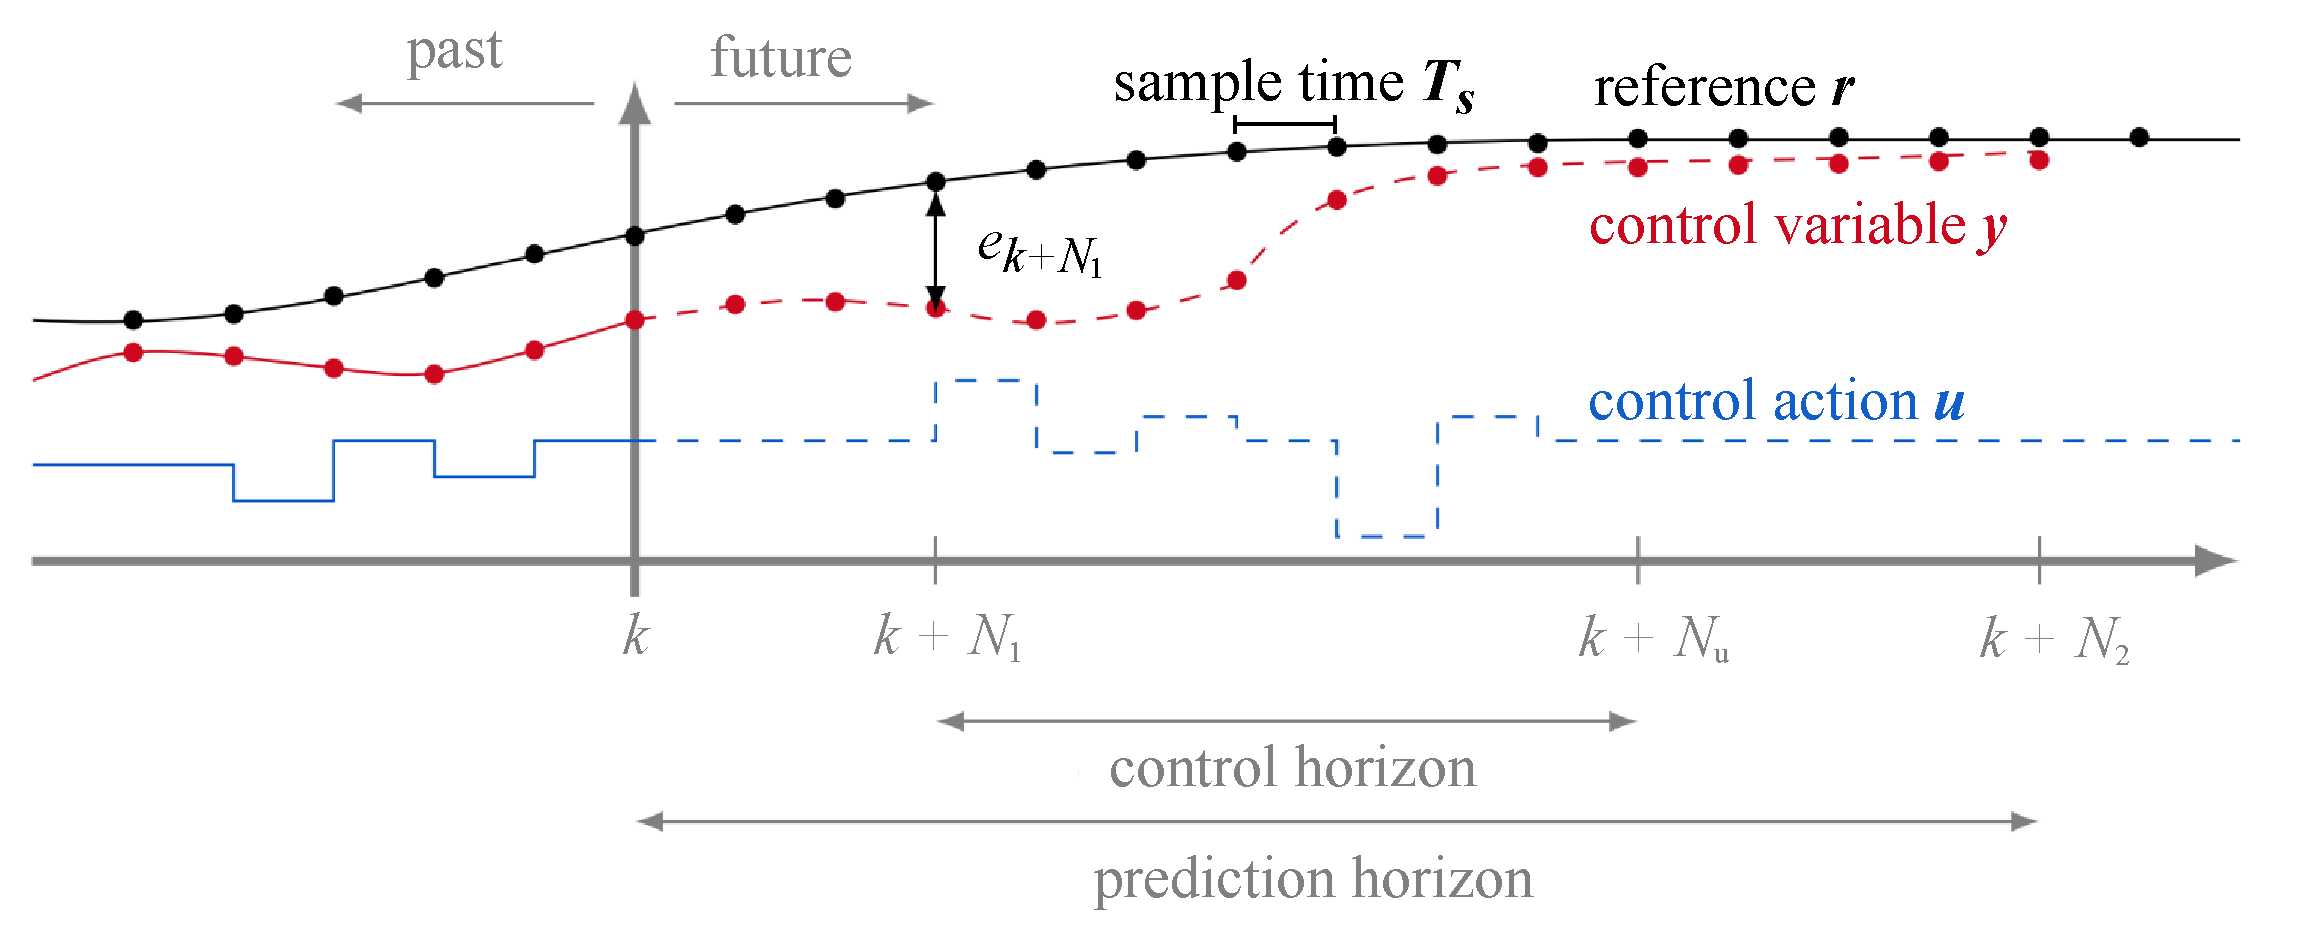
\includegraphics[width=1\textwidth]{fig/mpcprinciple}}
\caption[Funktionsprinzip eines MPC]{Funktionsprinzip eines MPC nach \cite[S.3]{Schwenzer} gemäß \cite{Richalet}}
    \label{fig_MPCVerhalten}
\end{figure}

\subsection{Modellierung des Systems} \label{subsec_Modellbildung}
Ein grundlegender Baustein zur erfolgreichen Regelung mit einem modellprädiktiven Regler ist die Abbildung des zu regelnden Systems durch mathematische Formeln – die Modellbildung.
Dabei kann das System sowohl in diskreter als auch kontinuierlicher Form vorliegen; für die Optimierung werden kontinuierliche Systeme aus Differenzialgleichungen und algebraischen Gleichungen jedoch in aller Regel diskretisiert, sodass das System letztlich wie in den Gleichungen \ref{eq_Modellbildung1} - \ref{eq_Modellbildung3} zu beschreiben ist.
Dabei steht $x$ für die dynamischen Modellzustände, $u$ für die Stellgrößen, $z$ für algebraische Größen und $p$ bzw.
$p_{tv}$ für (zeitabhängige, \textbf{t}ime \textbf{v}arying) Modellparameter. \cite[S.3]{Schwenzer}\cite{Dompc1}

\begin{equation} \label{eq_Modellbildung1}
    x_{k+1} = f(x_k, u_k, z_k, p_{tv,k}, p)
\end{equation}
\myequations{\quad Diskrete Zustandsgleichung in der Modellbildung}
\vspace*{-2.5\baselineskip}
\begin{equation} \label{eq_Modellbildung2}
    0 = g(x_k, u_k, z_k, p_{tv,k}, p)
\end{equation}
\myequations{\quad Gleichheitsbedingungen in der Modellbildung}
\vspace*{-2.5\baselineskip}
\begin{equation} \label{eq_Modellbildung3}
    y_k = h(x_k, u_k, z_k, p_{tv,k}, p)
\end{equation}
\centerline{\small{\textsf{\textbf{Formel \ref{eq_Modellbildung1} - \ref{eq_Modellbildung3}:}} Diskretisierte mathematische Modelldarstellung}}
\myequations{\quad Ausgangsgleichung in der Modellbildung}


\subsection{Kostenfunktion} \label{subsec_Modellbildung}
Liegt dem Controller ein mathematisch hinreichend beschriebenes Modell vor, kann eine sogenannte Kostenfunktion aufgestellt werden.
Während des Optimierungsprozesses wird der in Abbildung \ref{fig_RegelkreisMPC} dargestellte Optimizer diese Funktion minimieren.
In der Kostenfunktion sollte der Vergleich der zu regelnden Ausgangsvariablen mit der Referenztrajektorie über den Regelungshorizont in quadratischer Form abgebildet sein \cite[S.24]{Diehl}\cite[S.3]{Schwenzer}.
Weiterhin ist es zumeist zielführend die Veränderung der Eingangsvariablen in jedem Zeitschritt in die Kostenfunktion mit aufzunehmen, um einem ruckartigen Regelverhalten vorzubeugen.
Zuletzt ist es auch möglich einen Term in die Kostenfunktion einzubinden, welcher nicht über den gesamten Kontrollhorizont berechnet wird, sondern lediglich die abschließende Güte der Regelung bewertet \cite[S.24]{Diehl}.
Ein mathematisches Beispiel einer solchen Kostenfunktion ist in Formel \ref{eq_Kostenfunktion} zu sehen, dabei stehen $W_1$, $W_2$ und $W_u$ für Gewichtungsfaktoren und $y(k+i\rvert k)$ für die zum Zeitpunkt $k$ bezüglich des Zeitpunktes $k+i$ vorhergesagte Ausgangsvariable. \cite[S.3]{Schwenzer}

\begin{equation} \label{eq_Kostenfunktion}
    J = \sum_{i=N_1}^{N_2-1}\left(\lVert r(k+i\rvert k)-y(k+i\rvert k)\rVert_{W_1} + \Delta u_i^T W_u \Delta u_i\right) + \lVert r(N_2\rvert k)-y(N_2\rvert k)\rVert_{W_2}
\end{equation}
\centerline{\small{\textsf{\textbf{Formel \ref{eq_Kostenfunktion}:}} Beispielhafte Kostenfunktion für den MPC}}
\myequations{\quad Beispielhafte Kostenfunktion für den MPC}


\subsection{Constraints} \label{subsec_Constraints}
Wie in Abschnitt \ref{subsec_GrundlagenMPC} beschrieben, sind auch die Constraints, also Beschränkungen auf Inputs und Outputs des Systems, ein wesentliches Merkmal modellprädiktiver Regelung.
Während der Optimierung der Kostenfunktion wird bei Einbindung von Constraints sichergestellt, dass beispielsweise mechanische oder physikalische Limitierungen des Systems nicht überschritten werden.
Dabei ist zwischen den sogenannten \textit{hard constraints} und \textit{soft constraints} zu unterscheiden.
Nicht zu überschreitende, harte Limitierungen treten zumeist bei den Eingangsgrößen auf; beispielhaft kann das maximale Drehmoment eines Motors genannt werden.
Im Gegensatz dazu sind harte Beschränkungen auf Ausgangsgrößen eher nur gewünscht als wirklich erforderlich und können das Optimierungsproblem unlösbar machen.
Ein zusätzlicher Freiheitsgrad wird durch die Einführung von soft constraints und sogenannten \textit{Slack Variablen} $\xi$ geschaffen. \cite[S.4]{Schwenzer}

Mathematisch lässt sich die in Gleichung \ref{eq_Kostenfunktion} dann um die constraints auf das gesamte Optimierungsproblem erweitern (siehe \ref{eq_Optimierungsproblem}).
Dazu werden weitere Gewichtungsmatrizen nach \cite[S.4]{Schwenzer}$W_w$ und $W_\xi$ in der Kostenfunktion eingefügt, letztere als trade-off zwischen Dauer und Höhe der constraint Überschreitung \cite{Rawlings}.
Die Indizes \textit{lb} und \textit{ub} kennzeichnen die \textbf{l}ower bzw. \textbf{u}pper \textbf{b}ound, also die untere und obere Variablengrenze.

\begin{equation} \label{eq_Optimierungsproblem}
\begin{gathered}
    \min_{u, \xi} \quad (2.7)_{W_w}+\underbrace{\left\|_{\xi}(k+i \mid k)\right\|_{W_{\xi}}}_{\text {softening }} \qquad\\
    u_{l b} \leq(u(k+j \mid k)) \leq u_{u b}, \\
    y_{l b}-(\xi(k+i \mid k)) \leq(y(k+j \mid k)) \leq y_{u b}+(\xi(k+i \mid k)), \\
    \text { where } \xi \geq 0 \\
    \forall i \in\left\{N_1, \ldots, N_2-i\right\} \text { and } j \in\left\{0, \ldots, N_u\right\}
\end{gathered}
\end{equation}

\vspace*{-5.2\baselineskip}
\qquad subject to:
\vspace*{4.2\baselineskip}
\myequations{\quad Beispielhaftes Optimierungsproblem für den MPC}
\centerline{\small{\textsf{\textbf{Formel \ref{eq_Optimierungsproblem}:}} Beispielhaftes Optimierungsproblem für den MPC}}

Die durchdachte Aufstellung der Kostenfunktion ist für den Erfolg der Regelung unerlässlich; je besser diese an die Problemstellung und die gewünschte Lösung angepasst ist, desto größer sind die Erfolgsaussichten.


\section{Zielpunktregelung} \label{sec_Zielpunktregelung}
Neben der in Abschnitt \ref{subsec_Receiver} erwähnten Notwendigkeit der Zielpunktregelung zur Vermeidung zu hoher Temperaturen auf der Receiver-Front, ist ein weiteres wesentliches Ziel jener, die Maximierung des wirtschaftlichen Ertrags des Kraftwerkes.
Daher wird nachfolgend das daraus resultierende Optimierungsproblem erläutert sowie einige existierende Zielpunktregelungen aus der Literatur kurz vorgestellt.
Im Anschluss wird die in dieser Arbeit verwendete Strategie detaillierter beschrieben.

\subsection{Optimierungsproblem der Zielpunktregelung} \label{subsec_OptimierungZielpunkte}
Eine optimale Ausrichtung der Heliostaten wird erreicht, wenn die Temperatur an jedem Teil des Receivers gleich der maximal zulässigen Temperatur ist.
Aufgrund der Tatsache, dass ein Heliostat allerdings mit verschiedenen diskreten Teilen des Receivers, im folgenden \textit{Cups} genannt, korreliert, kann die Temperatur eines einzelnen Cups nicht durch einen Heliostaten angepasst werden, ohne die Temperatur der anderen Cups zu beeinflussen.
Aus diesem Grund kann es unmöglich sein, die perfekte Lösung zu finden, bei der an jedem Cup des Receivers die maximale Temperatur vorliegt.
Das Optimierungsproblem sollte also nicht auf die Temperatur der einzelnen Cups abzielen, sondern die insgesamt aufgenommene Leistung $P_{receiver}$ unter Einhaltung der Grenztemperatur maximieren.
Das zugehörige Optimierungsproblem ergibt sich dann gemäß Gleichung \ref{eq_OptimierungZielpunkte}, wobei $T_{absorber,i}$ die jeweilige Temperatur am Cup $i$ darstellt und $(x_{z,h}, y_{z,h})$ the Zielpunktkoordinaten eines jeden Heliostaten $h$ darstellen. \cite[S.15]{DissZanger}

\begin{equation} \label{eq_OptimierungZielpunkte}
\begin{gathered}
    \max \quad P_{\text {receiver }}  \qquad \\
    \begin{aligned}
        T_{front,i} \leq T_{front,max}, \qquad                 & \forall~i \in \left\{1, ..., n_{cups} \right\}       \\
        \left(x_{z,h}, y_{z,h}\right) \in \mathbb{R}^2, \qquad & \forall~h \in \left\{1, ..., n_{heliostats} \right\}
    \end{aligned}
\end{gathered}
\end{equation}

\vspace*{-2.95\baselineskip}
\qquad subject to:
\vspace*{1.95\baselineskip}
\myequations{\quad Kontinuierliches Optimierungsproblem der Zielpunktregelung}
\centerline{\small{\textsf{\textbf{Formel \ref{eq_OptimierungZielpunkte}:}} Kontinuierliches Optimierungsproblem der Zielpunktregelung}}

Wie bereits in Kapitel \ref{subsec_Modellbildung} erwähnt ist eine Diskretisierung des Modells zumeist hilfreich.
Die kontinuierliche Gleichung \ref{eq_OptimierungZielpunkte} erlaubt dem Heliostaten alle möglichen Zielpunkte in der Ebene $\mathbb{R}^2$.
Eine Diskretisierung durch Definition einer Teilmenge möglicher Zielpunktkoordinaten $A$ erlaubt eine mathematische Beschreibung des Problems wie in Gleichung \ref{eq_OptimierungZielpunkteDiskret}.

\begin{equation} \label{eq_OptimierungZielpunkteDiskret}
\begin{gathered}
    \max \quad P_{\text {receiver }}  \qquad \\
    \begin{aligned}
        T_{front,i} \leq T_{front,max}, \qquad      & \forall~i \in \left\{1, ..., n_{cups} \right\}       \\
        \left(x_{z,h}, y_{z,h}\right) \in A, \qquad & \forall~h \in \left\{1, ..., n_{heliostats} \right\}
    \end{aligned}
\end{gathered}
\end{equation}

\enlargethispage*{2\baselineskip}
\vspace*{-2.95\baselineskip}
\qquad subject to:
\vspace*{1.95\baselineskip}
\myequations{\quad Diskretes Optimierungsproblem der Zielpunktregelung}
\centerline{\small{\textsf{\textbf{Formel \ref{eq_OptimierungZielpunkteDiskret}:}} Diskretes Optimierungsproblem der Zielpunktregelung}}

Um die Streuung der Heliostaten möglichst gering zu halten und somit die Energieeffizienz des Kraftwerkes zu verbessern, werden die Heliostaten bevorzugt auf die Mitte gerichtet.
Werden jedoch alle Heliostaten auf die Mitte ausgerichtet, wird die zulässige Temperatur der Receiver-Front überschritten.
Welcher Heliostatenzielpunkt nun also in welche Richtung verschoben werden muss, hängt von dessen Standort ab.
Heliostaten, die einen kürzeren Abstand zum Receiver haben, streuen die Sonnenstrahlung über eine kleinere Fläche.
Da sie die gleiche Leistung reflektieren, aber über eine kleinere Fläche als weiter entfernte Heliostaten, erreichen Heliostaten, die näher am Receiver stehen, höhere maximale Flussdichten und haben größeren Einfluss auf die Temperatur einzelner Cups.

Es ist zu beachten, dass eine optimale Lösung des in Gleichung \ref{eq_OptimierungZielpunkteDiskret} formulierten Problems nicht notwendigerweise die optimale Lösung in Bezug auf das reale System ist, da das reale System Störungen unterworfen ist.
Die in Abschnitt \ref{subsec_OptischeVerluste} beschriebenen optischen Verluste sowie Wolken als meteorologische Einflüsse, wie in Abschnitt \ref{sec_Nowcasting} erwähnt, werden als Störgrößen betrachtet.
Sie verändern die Flussdichteverteilungen der Heliostaten und können daher die abgefangene Leistung einzelner Cups verringern oder auch erhöhen.
Durch den Tracking-Error beispielsweise könnte die erlaubte Temperatur des Receivers überschritten werden, wenn die Verschiebung hin zu einem bereits kritisch heißen Cup geschieht. \cite[S.16]{DissZanger}

Wolken reduzieren die reflektierte Strahlung während ihres Durchzuges, was die Möglichkeit bietet, die Zielpunkte weiter in Richtung Zentrum zu verschieben.
Zieht die Wolke weiter, während die Heliostaten immer noch stark in Richtung Receiver-Zentrum fokussieren, kann dies zu einer Überschreitung der maximalen Temperatur oder in dieser Arbeit nicht weiter betrachteter Temperaturgradienten führen.
Diesen Umstand zeigt umseitig die Abbildung \ref{fig_EinflussWolke}.
Hier wird ein konstanter Luftmassenstrom im Inneren des Receivers vorausgesetzt, sodass die Temperatur auf der Vorderseite ($T_{abs}$) und der Innenseite des Receivers $T_{outlet}$ lediglich von der solaren Einstrahlung $P_{solar}$ abhängig ist.
Die Details der Zusammenhänge dieser Größen werden in Kapitel \ref{sec_Ausgangszustand} beschrieben.

\enlargethispage*{\baselineskip}
\begin{figure}[h!]
    \centering
    \setlength{\fboxsep}{1pt}
    \setlength{\fboxrule}{1pt}
    \fbox{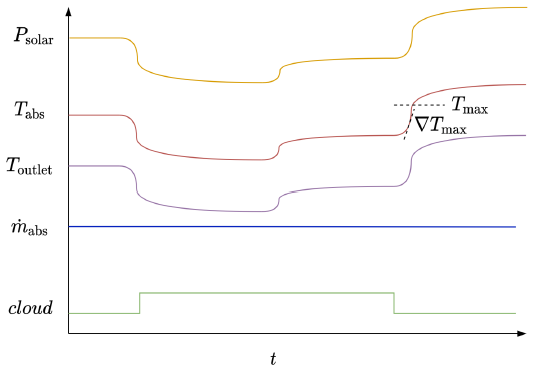
\includegraphics[width=0.75\textwidth]{fig/PassingCloud}}
    \caption[Darstellung der potenziellen Gefahr einer durchziehenden Wolke]{Darstellung der potenziellen Gefahr einer durchziehenden Wolke}
    \label{fig_EinflussWolke}
\end{figure}

\subsection{Existierende Algorithmen} \label{subsec_ZielpunktregelungLiteratur}
Eine präzise Übersicht über verschiedene Algorithmen zur Zielpunktregelung wurde von Oberkirsch in \cite{DissOberkirsch} aufgestellt.
An dieser Stelle werden beispielhaft einige dieser Regelungen kurz vorgestellt bevor nachfolgend in Absatz \ref{subsec_ZielpunktregelungGarcia} die in dieser Arbeit genutzte Zielpunktregelung detaillierter vorgestellt wird.

Maldonado \textit{et al.} \cite{Maldonado}\cite{Maldonado2} entwickelte beispielsweise einen iterativen Algorithmus mit dem Namen \textit{Local Search}.
Dieser beginnt bei einer initialen Lösung zur Zielpunktverteilung und untersucht für jeden Zeitschritt, ob eine Verschiebung zu diskreten benachbarten Zielpunkten im Hinblick auf die Gesamtleistung des Receivers einen Vorteil bringt.
Der jeweilige Heliostat ändert seine Ausrichtung dann so, dass die Leistung maximal gesteigert wird, sofern eine Steigerung möglich ist.
Auf diese Weise wird nach und nach über jeden benachbarten Zielpunkt und über alle Heliostaten iteriert.

In einer Arbeit von Cruz \textit{et al.} \cite{Cruz} wird ein Algorithmus zur Zielpunktsteuerung vorgeschlagen, der eine gewünschte Flussdichteverteilung auf dem Receiver erreichen soll.
Das Problem wird durch eine zweistufige Optimierung gelöst; die erste Stufe bestimmt mittels eines meta-heuristischen Algorithmus die zu optimierenden Heliostaten und die zweite Stufe legt mit einem gradientenbasierten Suchverfahren die Zielpunkte dieser Heliostaten fest. Erfolgreiche Tests dieses Verfahrens werden in der Veröffentlichung jedoch nur mit 50 aktiven Heliostaten beschrieben.


Vant-Hull \textit{et al.} \cite{VantHull2}\cite{VantHull3} hat unter anderem das \textit{Dynamic Aimpoint Processing System} (\textit{DAPS}) entwickelt; eine Regelung die im Wesentlichen das Überschreiten maximaler Flussdichten verhindern soll.
Dazu wird der Cup des Receivers mit der höchsten überschrittenen Flussdichte gemessen und simulativ bestimmt und anschließend identifiziert, welcher Heliostat den größten Einfluss auf diesen Cup nimmt; dieser Heliostat wird anschließend defokussiert.
In einem iterativen Prozess wird dieses Verfahren wiederholt, bis die Flussdichte an keinem Cup mehr überschritten wird.

García \textit{et al.} \cite{Garcia1} stellte einen Algorithmus vor, der das Problem nicht als MIMO System definiert, also mit allen Heliostaten als Eingangsgrößen und allen Zielpunkten als separat zu berechnende Ausgangsgrößen, sondern als System aus 6 \textit{SISO} (\textbf{S}ingle \textbf{I}nput \textbf{S}ingle \textbf{O}utput) Subsystemen.
Dazu werden die Heliostaten in drei Gruppen eingeteilt, je nach Entfernung zum Receiver.
Für jede Gruppe werden dann zwei Faktoren eingeführt: Ein Faktor, der das \textit{shifting}, also die Verschiebung der Zielpunktmitte jeder Gruppe vom Zentrum her beschreibt und einer, der die \textit{dispersion}, also die Streuung der Heliostaten von dieser Gruppenmitte ausangibt.
Auf diese Weise werden sechs Subsysteme gebildet, die von separaten \textit{PID}-Reglern geregelt werden.

Die Algorithmen, die nicht auf Basis einer Gruppierung von Heliostaten funktionieren, haben einen hohen Rechen- und Zeitaufwand in der Optimierung.
Weiterhin ist der DAPS-Algorithmus aufgrund anderer Nachteile für diese Arbeit ungeeignet; dazu zählt die Tatsache, dass er nicht für die Inbezugnahme von Wolken ausgelegt ist.
Darüber hinaus besteht die Notwendigkeit einer extrem präzisen Modellbildung, um den exakten Einfluss einzelner Heliostaten nutzen zu können und durch seinen Aufbau wird immer der Heliostat mit dem größten Einfluss manipuliert, welcher nicht zwangsläufig der ideale Heliostat in Bezug auf die Optimierung ist. \cite[S.35]{DissOberkirsch}
Die Einteilung des Systems in SISO-Subsysteme ist für stark gekoppelte Systeme mit großen Abhängigkeiten nicht sinnvoll. \cite[S.33]{DissZanger}


\subsection{Vorstellung des gewählten Algorithmus} \label{subsec_ZielpunktregelungGarcia}
Gewählt wird ein Algorithmus zur Zielpunktverteilung, welcher ebenfalls von Garcia \textit{et al.} \cite{Garcia2} vorgestellt wurde und mit Gruppierung von Heliostaten und der oben angesprochenen \textit{dispersion} der Heliostaten arbeitet.
Er ist ursprünglich für zylindrische Receiver gedacht, die Grundidee kann jedoch problemlos auf rechteckige Receiver übertragen werden.
Außerdem liegt auch bei diesem Ansatz der Fokus auf einer Regelung der maximal erlaubten Flussdichte; zu diesem Zweck wird ein Regelkreis mit einem MPC vorgestellt.
Für diese Arbeit wird jedoch lediglich der Algorithmus zur Bewegung der Zielpunkte benötigt und in das Modell des Solarturms Jülich eingebaut.
Daher kann die Regelung letztlich so durchgeführt werden, dass die maximal erlaubte Temperatur die Limitierung darstellt.
Von besonderer Relevanz ist also einerseits die Gruppierung der Heliostaten und andererseits das Verhalten der einzelnen Heliostaten innerhalb dieser Gruppe.

\subsubsection*{Gruppierung der Heliostaten} \label{subsubsec_Gruppierung}
Da García in seiner Forschung ein Rundum-Heliostatenfeld (vgl. Abschnitt \ref{subsec_Heliostaten}) untersucht, werden die Heliostaten zunächst in 18 Gruppen geteilt, die auf jeweils eins der 18 rechteckigen Teilstücke des insgesamt zylindrisch aufgebauten Receivers gerichtet werden.
Anschließend wird jede dieser Gruppen noch dreifach unterteilt.
Einerseits entstehen zwei Gruppen mit einem Radius von $<400m$ Entfernung zum Receiver, welche im gleichen Teil des Feldes stehen und eine ähnliche Leistung zum Receiver reflektieren können.
Die dritte Gruppe umfasst alle weiteren Heliostaten mit größerem Abstand zum Receiver. \cite[S.8-10]{Garcia2}\\
Abbildung \ref{fig_VerteilungHeliostateGarcia} zeigt diese Einteilung in 18x3 Gruppen von Heliostaten; die Gruppen sind farblich in Rot, Grün und Blau dargestellt.

\begin{figure}[h!]
    \centering
    \setlength{\fboxsep}{1pt}
    \setlength{\fboxrule}{1pt}
    \fbox{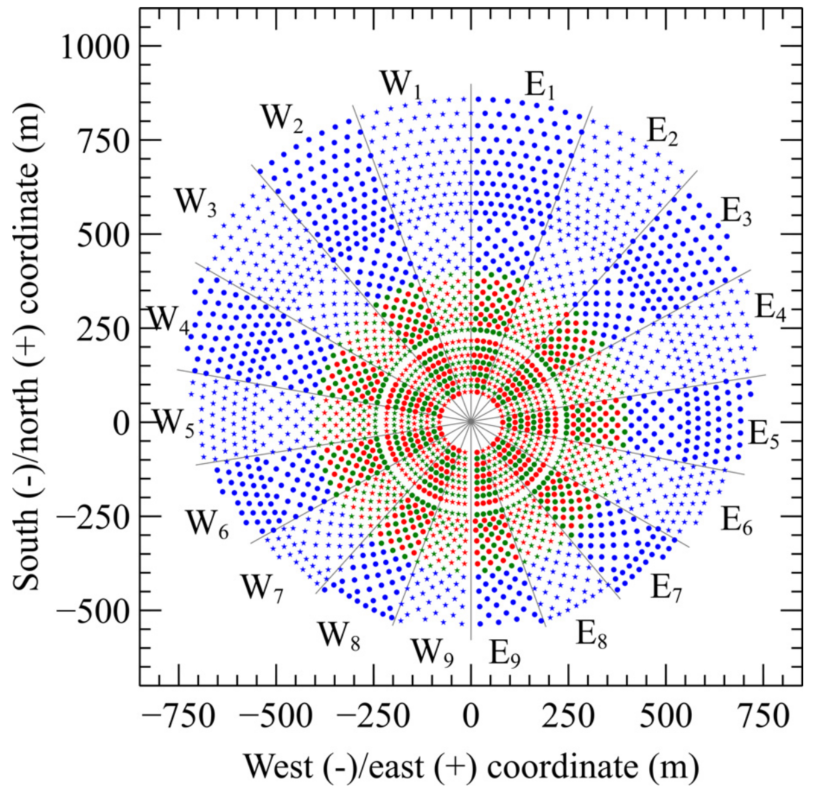
\includegraphics[width=0.6\textwidth]{fig/GarciaFeld}}
\caption[Einteilung des Heliostatenfeldes des Gemasolar-Kraftwerkes in Sevilla in 54 Gruppen]{Einteilung des Heliostatenfeldes des Gemasolar-Kraftwerkes in Sevilla in 54 Gruppen \cite[S.10]{Garcia2}}
    \label{fig_VerteilungHeliostateGarcia}
\end{figure}

Für die vorliegende Arbeit entfällt die Unterteilung in 18 Gruppen aufgrund der Receiver- und Heliostatenfeldstruktur, sodass das gesamte Feld in lediglich drei Teile eingeteilt wird.
Weiterhin unterscheiden sich in dieser Ausarbeitung auch die erste und zweite Gruppe in der Distanz bezogen auf den Receiver, wie in Kapitel \ref{sec_ErweiterungModellbildung} erläutert wird.

\subsubsection*{Verhalten der Heliostaten innerhalb einer Gruppe} \label{subsubsec_Gruppenverhalten}
Das von Garía vorgestellte Verfahren besitzt zwei Parameter, um das Verhalten der einzelnen Heliostaten innerhalb der Gruppe zu beeinflussen.
Einerseits den \textit{dispersion factor} $\kappa$, der Auskunft über die Streuung der Heliostaten innerhalb der Gruppe gibt und andererseits den Parameter $y_{Cent}$, der die vertikale Position des \gans{Schwerpunktes} aller Zielpunkte auf dem Receiver beeinflussen kann \cite[S.5]{Garcia2}.
Zweiterer ist bei zylindrischen Parametern notwendig, kann aber nachfolgend vernachlässigt werden und wird zu $y_{Cent} = 0$ gesetzt.
Da sowohl nachfolgend als auch in der Arbeit von García $x_{Cent} = 0$ gilt, wird sichergestellt, dass der Schwerpunkt aller drei betrachteter Gruppen im Zentrum des Receivers bei $(0,0)$ liegt.
Abbildung \ref{fig_DispersionVeranschaulichung} zeigt den Einfluss der beiden Stellgrößen exemplarisch, wobei erkennbar ist, dass $\kappa_1 > \kappa_2$, da die Streuung an dieser Stelle größer ist.

\begin{figure}[h!]
    \centering
    \setlength{\fboxsep}{1pt}
    \setlength{\fboxrule}{1pt}
    \fbox{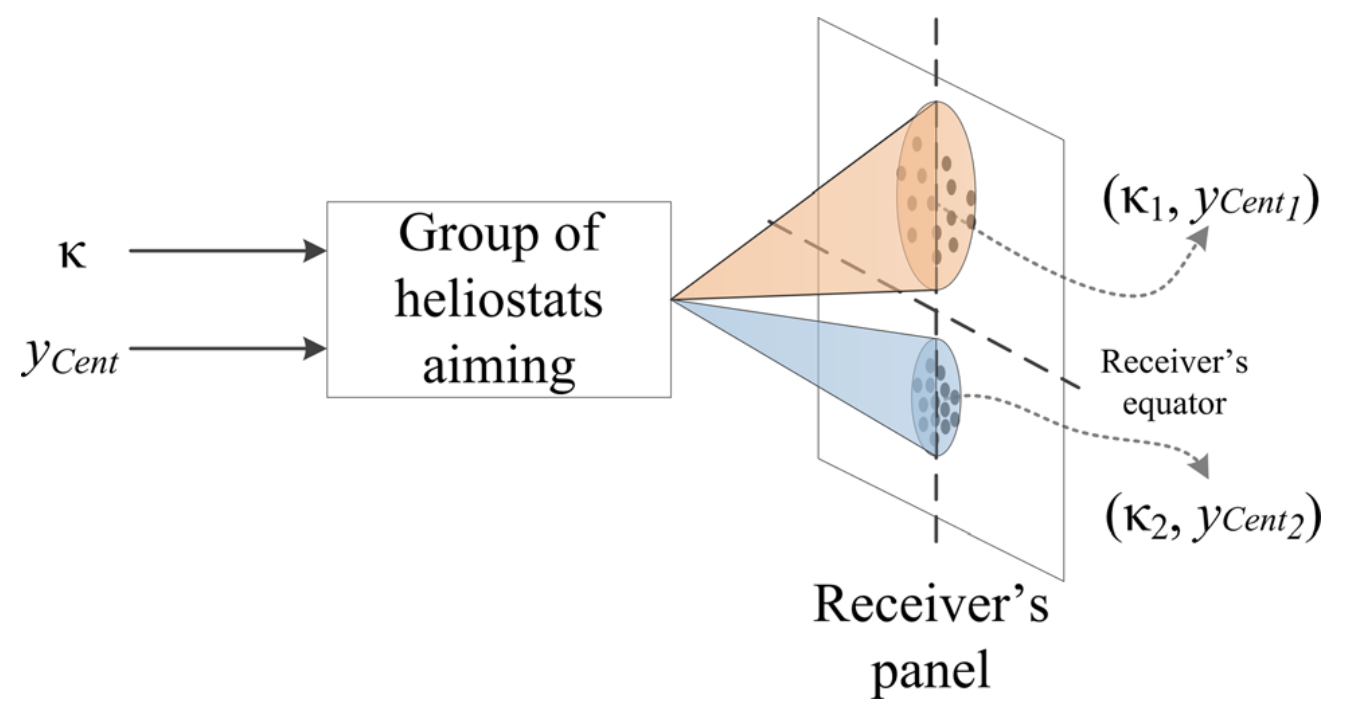
\includegraphics[width=0.6\textwidth]{fig/GarciaDispersionSymbolisch}}
\caption[Symbolische Veranschaulichung der Stellgrößen des gewählten Algorithmus]{Symbolische Veranschaulichung der Stellgrößen des gewählten Algorithmus \cite[S.7]{Garcia2}}
    \label{fig_DispersionVeranschaulichung}
\end{figure}


Die Zielpunkte der Gruppe werden letztlich zwei Kriterien erfüllen, wenn der vorgestellte Algorithmus die Stellgrößen $\kappa$ und $y_{cent}$ verwertet und sich ein Gleichgewichtszustand eingestellt hat:
\begin{itemize}
    \item Jeder einzelne Punkt wird so nah wie möglich am festgelegten Schwerpunkt der Gruppe sein und dabei einen individuellen Minimalabstand zum nächsten Zielpunkt $r$, welcher von $\kappa$ abhängt, nicht unterschreiten.
    \item Ihr Gruppenschwerpunkt wird mit dem durch $(x_{cent}, y_{cent})$ vorgegebenen Punkt, hier also $(0,0)$, übereinstimmen.
\end{itemize}

\textit{Kriterium 1:}\\
Ein statischer Parameter $a$ wird verwendet, um die Heliostaten einer Gruppe zu organisieren. Dieser Parameter weist jedem Heliostaten individuell einen Wert $\alpha$ zu, welcher sich aus der Anzahl der Heliostaten $n$ und $a$ ergibt (siehe Gleichung \ref{eq_GarciaAlpha} und \ref{eq_GarciaDeltaAlpha}).

\begin{gather}
    \alpha \in \left[-a, -a+\Delta\alpha, -a+2\Delta\alpha,..., a\right] \label{eq_GarciaAlpha}\\
    \text{\myequations{\quad Berechnung des individuellen Heliostatenparameters $\alpha$}}
    \text{Mit:\qquad}\Delta\alpha = \frac{2\alpha}{n-1}, \quad \forall~\left\{n \in \mathbb{N} \mid x > 1 \right\} \qquad\qquad \label{eq_GarciaDeltaAlpha}
\end{gather}
\centerline{\small{\textsf{\textbf{Formel \ref{eq_GarciaAlpha} und \ref{eq_GarciaDeltaAlpha}:}} Berechnung des individuellen Heliostatenparameters $\alpha$}}
\myequations{\quad Berechnung von $\Delta\alpha$}

Daraus kann für jeden Heliostaten der Radius $r$ berechnet werden, der den Mindestabstand zu benachbarten Zielpunkten vorgibt.
Er ergibt sich gemäß \ref{eq_GarciaMindestabstand}, wobei $\kappa$ wie beschrieben die Stellgröße des Controllers zur Zielpunktstreuung darstellt und $\beta$ ein Skalierungsfaktor ist.

\begin{equation} \label{eq_GarciaMindestabstand}
    r=\frac{\kappa}{1+\left|\frac{\alpha}{\kappa}\right|^{2\kappa}}\cdot\beta
\end{equation}
\begin{center}
    \begin{varwidth}{0.95\textwidth}
\small{\textsf{\textbf{Formel \ref{eq_GarciaMindestabstand}:}} Bestimmung des Mindestabstandes eines jeden Zielpunktes zum nächstgelegenen Zielpunkt der Heliostatengruppe}
    \end{varwidth}
\end{center}
\myequations{\quad Bestimmung des Mindestabstandes eines jeden Zielpunktes zum nächstgelegenen\\\hspace*{0.3cm} Zielpunkt der Heliostatengruppe}

Abbildung \ref{fig_Verteilunglpha} zeigt die sich ergebenden Radien je nach individuellem $\alpha$-Wert exemplarisch für $\kappa=2$ bzw. $\kappa=5$.
Es ist erkennbar, dass die Wahl hoher Werte für $a$ kleine Abstände zwischen den Zielpunkten zur Folge haben wird.

\begin{figure}[h!]
    \centering
    \setlength{\fboxsep}{1pt}
    \setlength{\fboxrule}{1pt}
    \fbox{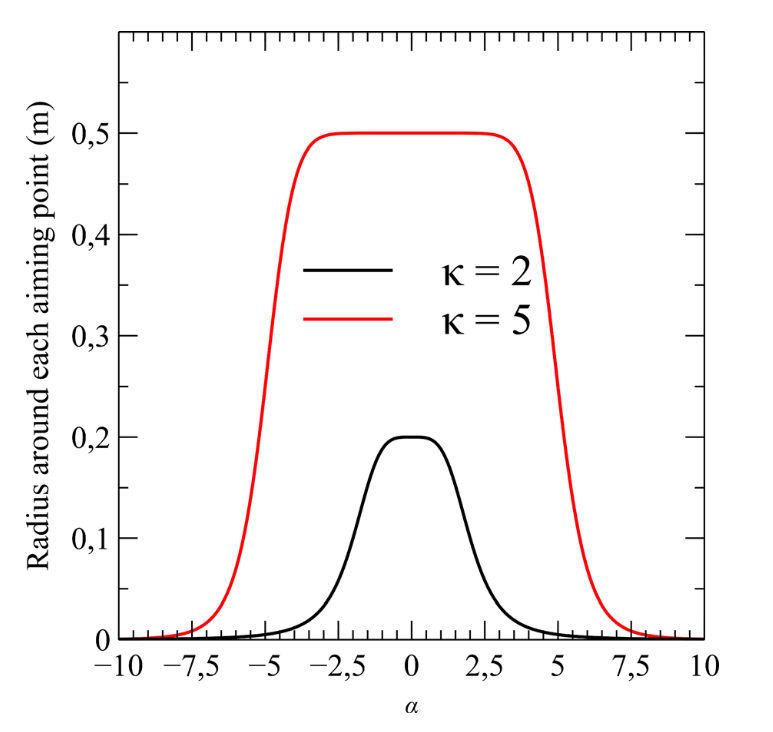
\includegraphics[width=0.5\textwidth]{fig/GarciaVerteilungAlpha.png}}
\caption[Minimalabstände der Zielpunkte je $\alpha$-Wert]{Minimalabstände der Zielpunkte je $\alpha$-Wert \cite[S.9]{Garcia2}}
    \label{fig_Verteilunglpha}
\end{figure}

Auf den durch $\kappa$ festgelegten Mindestabständen aufbauend, ergeben sich, sofern noch kein Gleichgewichtszustand erreicht ist, Bewegungen der Heliostaten und Zielpunkte.
Die Distanz, die zwischen zwei Zielpunkten zurückgelegt werden muss, ist in der Arbeit mit $\Delta D$ benannt und setzt sich aus $\Delta x$ und $\Delta y$ zusammen; Strecken in beiden Dimensionen, die auf dem Receiver zwischen zwei Zielpunkten zurückgelegt werden müssen.
Die Arbeit von García präsentiert außerdem die Berechnungsvorschrift, aus der hervorgeht, wie weit sich jeder einzelne der beiden Zielpunkte nun in beide Richtungen bewegen muss \cite[S.9-10]{Garcia2}.
Um sicherzustellen, dass der Abstand eines jeden Zielpunktes zu allen anderen Zielpunkten der Gruppe eingehalten wird, wiederholen sich diese Berechnungsvorschriften für jedes mögliche Pärchen aus Heliostaten \cite[S.9]{Garcia2}.
Anschließend wird der Durchschnitt der berechneten Distanzen eines Zielpunktes relativ zu den anderen Heliostaten ($\overline{\Delta x_{TP_i}}$) und ($\overline{\Delta y_{TP_i}}$) errechnet \cite[S.10]{Garcia2}.


\textit{Kriterium 2:}\\
Wie erläutert, kommt es nun also zu erforderlichen Bewegungen der Zielpunkte auf dem Receiver.
Diese Bewegungen müssen nun so reguliert werden, dass der Schwerpunkt der Heliostatengruppe weiterhin dem vorgegebenen Gruppenmittelpunkt übereinstimmt.
Dazu wird $\Delta D_{Centroid}$ bestimmt, ein Wert der angibt wie weit sich das Gruppenzentrum vom geforderten Punkt unterscheidet.
Er berechnet sich nach Gleichung \ref{eq_GarciaGruppenzentrumbewegung}, wobei $k_2$ eine Konstante zur Berücksichtigung der zulässigen Stellgeschwindigkeiten der Heliostaten darstellt. \cite[S.10]{Garcia2}

\begin{equation} \label{eq_GarciaGruppenzentrumbewegung}
    \Delta D_{Centroid} = k_2 \cdot \sqrt{\left(x_{Cent}-x_{Actual Centroid}\right)^2+\left(y_{Cent}-y_{Actual Centroid}\right)^2}
\end{equation}
\centerline{\small{\textsf{\textbf{Formel \ref{eq_GarciaGruppenzentrumbewegung}:}} Erforderliche Schwerpunktverschiebung der Zielpunktgruppe}}
\myequations{\quad Erforderliche Schwerpunktverschiebung der Zielpunktgruppe}

Darauf aufbauend ergeben sich mathematisch erneut die erforderlichen Verschiebungen der Gruppe $\Delta X_{Group}$ und $\Delta Y_{Group}$ nach \cite[S.10]{Garcia2}.
Zuletzt können die tatsächlichen Koordinaten eines jeden Zielpunktes im nächsten Zeitschritt durch Verschiebung der vorigen Koordinaten um $\overline{\Delta x,y_{TP_i}}$ und $\overline{\Delta X,Y_{Group}}$ bestimmt werden.
Die vollständige Darstellung des hier vorgestellten Algorithmus nach García \textit{et al.} \cite{Garcia2} zeigt demnach Abbildung \ref{fig_GarciaAlg}.

\begin{figure}[p]
    \centering
    \setlength{\fboxsep}{1pt}
    \setlength{\fboxrule}{1pt}
\fbox{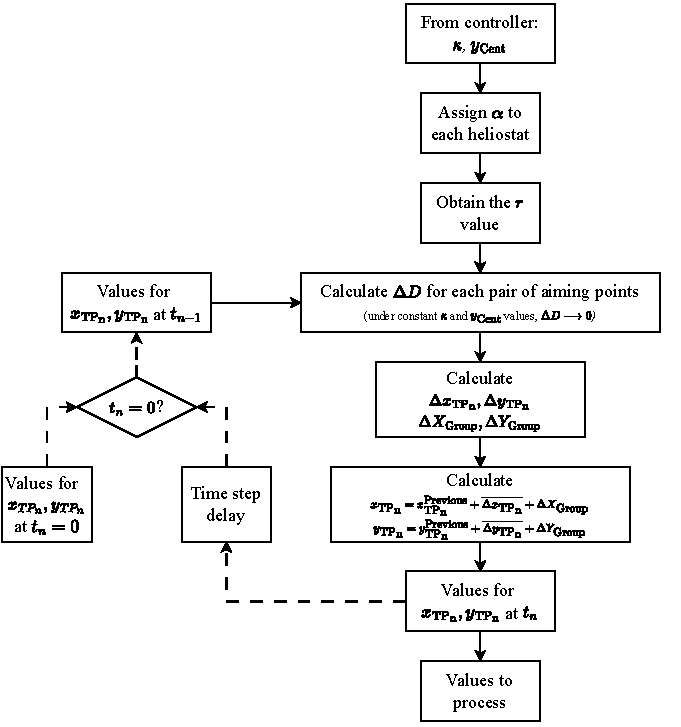
\includegraphics[width=0.9\textwidth]{fig/AlgorithmusGarcia.pdf}}
\caption[Übersicht der vollständigen Zielpunktstrategie nach García]{Übersicht der vollständigen Zielpunktstrategie nach García \cite[S.10]{Garcia2}}
    \label{fig_GarciaAlg}
\end{figure}

Eine beispielhafte Zielpunktverteilung für einen zunehmenden Faktor $\kappa$ und einem Gruppenzentrum in der Mitte des Receivers ist umseitig in Abbildung \ref{fig_GarciaZielpunkte} erkennbar.
Es wird deutlich, dass das Gruppenzentrum nach wie vor in der Mitte liegt und die Abstände zwischen den Zielpunkten dennoch sichtbar zunehmen.
Aufgrund des individuellen Parameters $\alpha$ sind die erforderlichen Mindestabstände jedoch nicht für alle Zielpunkte gleich groß.

\begin{figure}[h!]
    \centering
    \setlength{\fboxsep}{1pt}
    \setlength{\fboxrule}{1pt}
    \fbox{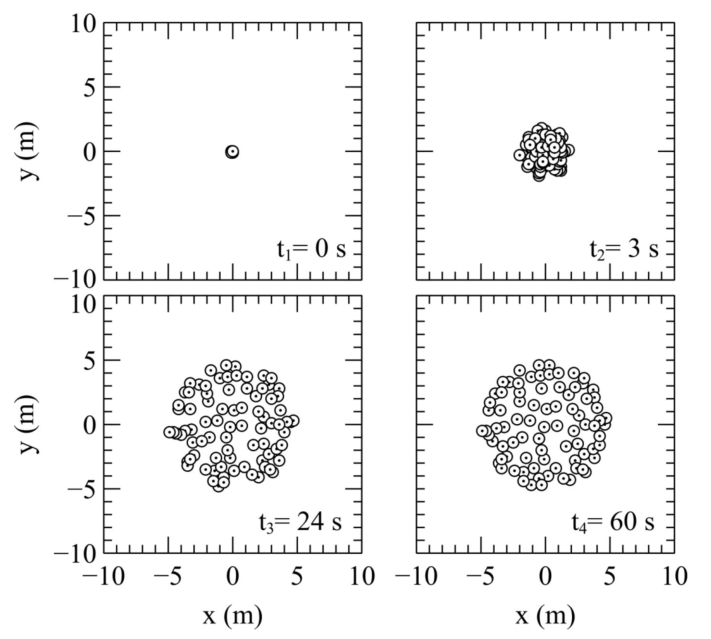
\includegraphics[width=0.75\textwidth]{fig/GarciaZielpunkte}}
\caption[Beispielhafte Zielpunktverteilungen für einen zunehmenden $\kappa$ Wert]{Beispielhafte Zielpunktverteilungen für einen zunehmenden $\kappa$ Wert \cite[S.11]{Garcia2}}
    \label{fig_GarciaZielpunkte}
\end{figure}

\subsubsection*{Zusammenfassung} \label{subsubsec_Zusammenfassung}
Letztlich handelt es sich bei dem vorgestellten Algorithmus von García um eine Strategie, um viele Heliostaten mit einer geringen Anzahl an Stellgrößen auf individuellen Bahnen zu bewegen.
Dafür werden pro Gruppe lediglich zwei Stellgrößen eingeführt, von der im Verlauf der Arbeit nur noch eine weiter betrachtet wird.
Ein wesentlicher Vorteil des gewählten Algorithmus ist die enorme Reduzierung der Stellgrößen; statt die vorhandenen 2153 Heliostaten am Standort Jülich einzeln positionieren zu müssen, geschieht dies durch lediglich 3 Stellgrößen.
Außerdem stehen als Endergebnis der Berechnung die einzelnen Zielpunkte der Heliostaten zur Verfügung.
Dies sorgt für eine gute Kompatibilität in der Modellbildung des gesamten Systems, wie es in Kapitel \ref{sec_ErweiterungModellbildung} erläutert wird.


\section{Verwendete Hard- und Software} \label{sec_HardSoftware}
Die Modellbildung und die Simulationen in den nachfolgenden Kapiteln werden mithilfe der Programmiersprache \textit{Python} umgesetzt.
Dabei handelt es sich Stand März 2023 um die populärste Programmiersprache weltweit \cite{Statista}.
Nicht zuletzt aufgrund der Echtzeitfähigkeit \cite[S.9]{Python} und einfachen Syntax hat es sich besonders im Bereich des \textit{machine learning}s als Stand der Technik etabliert.
Darüber hinaus zeichnet sich Python durch seine große Anzahl an professionellen Frameworks und Bibliotheken aus, welche es Entwicklern ermöglichen, auch komplexe Probleme mit geringem Aufwand zu lösen \cite[S.3]{Python}.
Zwei wesentliche Beispiele für solche Frameworks, die auch in dieser Arbeit Verwendung finden sind \gans{CasADi} und \gans{do-mpc}.

CasADi ist eine Open-Source Bibliothek für MATLAB/Octave, C++ und Python.
Sie dient der gradientenbasierten numerischen Optimierung mit einem besonderen Fokus auf der Regelungstechnik.
Durch CasADi soll besonders die symbolische Formulierung von gewöhnlichen Differentialgleichungen (ODEs) und differential-algebraischen Gleichungen (DAEs) erleichtert und damit die Formulierung und Lösung nicht-linearer Programme und Regelungsprobleme ermöglicht werden. \cite{Casadi}

Do-mpc ist ebenfalls eine Open-Source Toolbox.
Sie basiert auf CasADi und ermöglicht die einfache Handhabung von Problemen mit Modellprädiktiven Regelung und der Zustandsvorhersage mittels \textit{moving horizon estimation} (MHE).
Ihre Modelle vereinen modular Simulations- Vorhersage- und Regelungskomponeten aus diesem Bereich \cite{Dompc2}.
Die gesamte Modellbildung, wie sie nachfolgend in Kapitel \ref{ch_Modellbildung} beschrieben ist, wird in do-mpc realisiert und ausgewertet.

Für die Simulation der Ergebnisse wird in dieser Arbeit ein 4-Kern Intel Core i7-1185G7 Prozessor mit einem Basistakt von 3,0 GHz verwendet.
Als Arbeitsspeicher stehen 16 GB RAM mit 4267 MHz zur Verfügung.
Das Betriebssystem ist Windows 10 Enterprise (Version 21H2).
